% ==============================================
% CFD Tutorial Template: OpenFOAM Terminal Basics
% Class: scrartcl (KOMA-Script) - optimized for tutorials
% Content: pitzDaily with simpleFoam
% ==============================================

\documentclass[
parskip=half,      % Space between paragraphs (better for steps)
DIV=12,            % Optimal margins for readability
headings=normal,   % Professional heading sizes
fontsize=11pt,     % Slightly larger for screen reading
english            % Language setting
]{scrartcl}

\input{../preamble.tex}
\usepackage{twemojis}
\usepackage{amssymb}

% ========== DOCUMENT START ==========
\begin{document}
	
	% ========== TITLE PAGE ==========
	\title{Tutorial \#6: 3D Y-Pipe and Turbulence Models}
	\subtitle{Incompressible Steady Flow: 3D Y-Pipe with different turbulence models}
	\subject{Open Source CFD }
	\author{Robert Castilla \\ Department of Fluid Mechanics}
	\date{2025-26 \\ Version 1.0}
	\publishers{Learning Objectives:
		\begin{itemize}
			\item Switch between turbulence models in CfdOF
			\item Understand the $y^+$ parameter and its importance
			\item Compute and visualize $y^+$ directly in ParaView
			\item Compare laminar, $k$-$\varepsilon$, $k$-$\omega$ SST, and SSTLM models
			\item Determine if mesh is appropriate for each model using $y^+$
			\item Analyze how turbulence affects flow separation and mixing
		\end{itemize}}
	
	\maketitle
	
	% ========== ABSTRACT ==========
	\begin{abstract}
		This tutorial explores turbulence modeling using the Y-pipe geometry from Tutorial \#5. 
		Instead of editing dictionaries manually, you will use CfdOF's intuitive GUI to switch 
		between turbulence models. You will learn how the $y^+$ parameter 
		determines whether your mesh is suitable for each model, and how to visualize $y^+$ in 
		ParaView. By the end, you'll understand why the same mesh can be perfect for one model 
		and completely inadequate for another.
	\end{abstract}
	
	\tableofcontents
	\newpage
	
	\section{Introduction to Turbulence Modeling in CfdOF}
	
	\subsection{Why Turbulence Models Matter}
	
	Most engineering flows are turbulent. The choice of turbulence model affects:
	
	\begin{itemize}
		\item \textbf{Predicted pressure drop} (important for pump sizing)
		\item \textbf{Flow separation} (recirculation zones, mixing)
		\item \textbf{Mesh requirements} ($y^+$ constraints determine cell size near walls)
		\item \textbf{Computational cost} (more equations = slower)
	\end{itemize}
	
	\subsection{Turbulence Models in CfdOF}
	
	CfdOF provides easy access to these RANS models:
	
	\begin{table}[h]
		\centering
		\begin{tabular}{|l|l|l|l|}
			\hline
			\textbf{Model} & \textbf{CfdOF menu option} & \textbf{Equations} & \textbf{$y^+$ requirement} \\
			\hline
			Laminar & "Laminar" & 0 & N/A \\
			Standard $k$-$\varepsilon$ & "RANS k-epsilon" & 2 & $> 30$ (wall functions) \\
			$k$-$\omega$ SST & "RANS k-omega SST" & 2 & $< 1$ or $> 30$ \\
			SSTLM & "RANS k-omega SSTLM" & 4 & $< 1$ (must resolve transition) \\
			\hline
		\end{tabular}
		\caption{Turbulence models available in CfdOF}
		\label{tab:models}
	\end{table}
	
	\subsection{The Critical Concept: $y^+$}
	
	$y^+$ is the dimensionless wall distance:
	
	\begin{equation}
		y^+ = \frac{y u_\tau}{\nu}
	\end{equation}
	
	where $u_\tau = \sqrt{\tau_w/\rho}$ is the friction velocity.
	
	The dimensionless velocity $u^+$ is function of the dimensionless distance to wall. For a turbulent boundary layer, it is assumed, and experimentally 
	validated that the function is linear, 
	\begin{equation}
		u^+ = y^+
	\end{equation}
	close to the wall ($y^+ \lessapprox 5$), and it follows a logarithm law,
	\begin{equation}
		u^+ = B + \frac{1}{\kappa}\log(y^+)
	\end{equation}
	, where $B\approx5$ and $\kappa\approx0.42$, at a distance $y^+ \gtrapprox 30$ (see Figure \ref{fig:lawofthewall}). For high Reynolds number, mesh the domain near the wall to get small values of 
	$y^+$ can be very expensive in term of computational resources and time 
	(very large mesh). This computation is avoided with the use of 
	a \texttt{\textbf{Wall Function}} that models the behavior of the 
	flow as far as $y^+$ is large enough, in the log-law region. The buffer region, $5 \lessapprox y^+ \lessapprox 30$ should be, in general, avoided. 
	
	
\begin{figure}[h]
	\centering
	
	\label{fig:lawofthewall}
	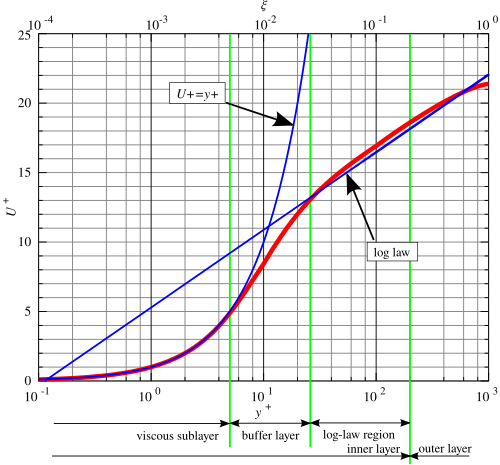
\includegraphics[width=0.5\linewidth]{Law_of_the_wall}
	\caption{Law of the wall showing $y^+$ regions. From \href{https://en.wikipedia.org/wiki/Law_of_the_wall}{WikiPedia}}
\end{figure}
	
%	\important{The mesh from Tutorial \#5 has $y^+ \approx 30-50$ on the walls. This is:
%		\begin{itemize}
%			\item  \textbf{Perfect} \texttwemoji{check mark button} for $k$-$\varepsilon$ with wall functions
%			\item  \textbf{Acceptable} \texttwemoji{warning} for $k$-$\omega$ SST in wall-function mode
%			\item  \textbf{Inadequate} \texttwemoji{x} for SSTLM (needs $y^+ < 1$)
%	\end{itemize}}
	
	\section{Computation of $y^+$ for the $k-\omega$ SST simulation}
	
	In tutorial \#5 we have performed the simulation with the $k-\omega$ SST turbulence model. Now we are going to perform the rest of simulations (Laminar, $k-\varepsilon$, $k-\omega$ SSTLM) in the same document. But, first, let's compute the value of $y^+$ for the simulation already done.
	
	\subsection{Setup of the \texttt{FreeCAD-CfdOf} session}
	
	
	\begin{itemize}
		\item Load the FreeCAD project from Tutorial \#5 and save it as \texttt{Tutorial\_6} in the proper folder.
		\item Change the \texttt{default output directory} in \texttt{CfdOf preferences} to the Tutorial \#6 folder 
		\item Let's we tell \texttt{FreeCAD} to allow duplicate names in the tree. Open \texttt{Edit $\rightarrow$ Preferences} and, in \texttt{General/Document} check on the box for \texttt{Allow duplicate object labels in one document}. Close with \texttt{OK}
	\end{itemize}
	 
	\subsection{Making again the $k-\omega$ SST simulation}
	
	\begin{itemize}
		\item Rename the \texttt{CfdAnalysis} as \texttt{Ypipe\_kOmegaSST}
		% TODO: \usepackage{graphicx} required
		\begin{figure}
			\centering
			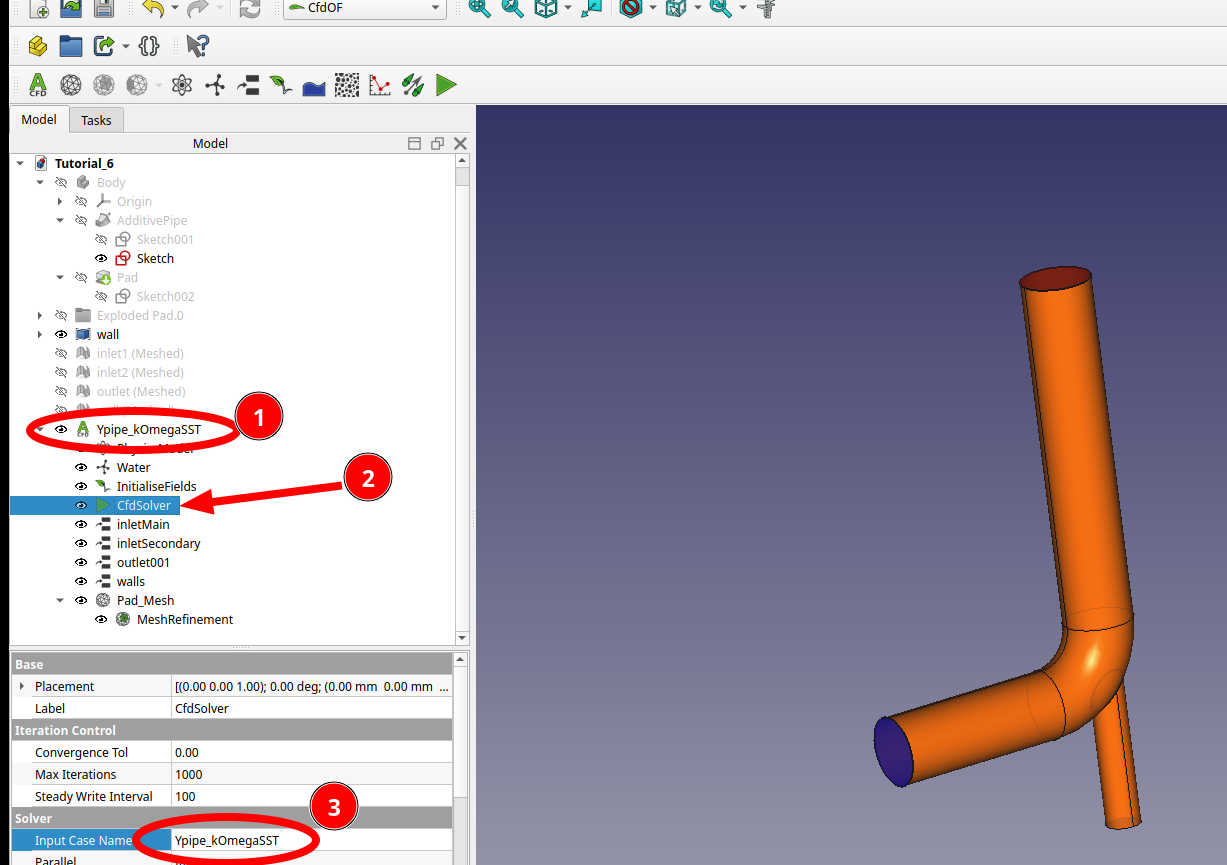
\includegraphics[width=0.7\linewidth]{change_names}
			\caption{Changing names in the initial simulation}
			\label{fig:changenames}
		\end{figure}
		
		\item \texttt{Write} and \texttt{Run} the case so that we will have it available in our new folder for Tutorial \#6. 
		\item The simulation can be stopped in 500 iterations, since the result
		will be almost the definitive one.
	\end{itemize}
	
	\subsection{Estimation of $y^+$ with CLI}
	\begin{itemize}
		\item In the \texttt{Analysis control} window click on \texttt{Edit} to open the file \texttt{File Manager} and with the right-button in the mouse select \texttt{Open in Terminal}. Alternatively, a terminal can be open with \texttt{ctrl-alt-t} and then navigate to the simulation's case. You should be in 
		
		\begin{lstlisting}[style=output ]
eseiaat@eseiaat-linux:~/Tutorials/Tutorial_6/Ypipe_kOmegaSST$
		\end{lstlisting}
	
	
		\item Load \texttt{OpenFOAM}
		
		\begin{lstlisting}[style=terminal]
source /usr/lib/openfoam/openfoam2312/etc/bashrc
		\end{lstlisting}
		
		\tip{Remember the \texttt{tab} autocompletion.}
		
		\item Get the dictionary to compute $y^+$.
		\begin{lstlisting}[style=terminal]
foamGetDict yPlus
		\end{lstlisting}
		
		\item Run the \texttt{yPlus} function
		\begin{lstlisting}[style=terminal]
simpleFoam -postProcess -func yPlus -latestTime
		\end{lstlisting}
		
		You will get the main information of the computation, similar to the output of Listing \ref{lst:yPlus}, and also a new file \texttt{yPlus}
		will be in the folder for the latest simulation time, e.g. \texttt{500}. 
		
		\begin{lstlisting}[style=output,caption={Output of \texttt{yPlus}} function, label={lst:yPlus}]
Create time

Create mesh for time = 500


SIMPLE: convergence criteria
field "(p|p_rgh)"	 tolerance 0.001
field U	 tolerance 0.001
field "(k|epsilon|omega|f|v2|nuTilda|gammaInt|ReThetat)"	 tolerance 0.001

Time = 500
Reading field p

Reading field U

Reading/calculating face flux field phi

Selecting incompressible transport model Newtonian
Selecting turbulence model type RAS
Selecting RAS turbulence model kOmegaSST
Selecting patchDistMethod meshWave
RAS
{
	RASModel        kOmegaSST;
	turbulence      on;
	printCoeffs     on;
	alphaK1         0.85;
	alphaK2         1;
	alphaOmega1     0.5;
	alphaOmega2     0.856;
	gamma1          0.555555555555556;
	gamma2          0.44;
	beta1           0.075;
	beta2           0.0828;
	betaStar        0.09;
	a1              0.31;
	b1              1;
	c1              10;
	F3              false;
	decayControl    false;
	kInf            0;
	omegaInf        0;
}

No MRF models present

No finite volume options present
yPlus yPlus write:
writing field yPlus
patch walls y+ : min = 1.91730240538628, max = 258.340024080099, average = 41.7649846515448

End	
		\end{lstlisting}
		
		\tip{The \texttt{yPlus} function, which calculates $y^+$ at the domain wall, supports many options. In this tutorial, the default settings are used, but you can view all of them on \href{https://doc.openfoam.com/2312/tools/post-processing/function-objects/field/yPlus/}{openfoam.com}  }
		
		\item Click on \texttt{ParaView} in \texttt{FreeCAD} to open the results for the last time. Choose in the \texttt{OpenFOAMReader1} element just the \texttt{wall} patch
		
		\item Apply the \texttt{Threshold Filter} to show only the values of $y^+$ between 5 and 30. The size of the wall with these values is very large, as shown in Figure \ref{fig:yplus1}. This could be the reason 
		of the poor convergence of the simulation,
		
		% TODO: \usepackage{graphicx} required
		\begin{figure}[h]
			\centering
			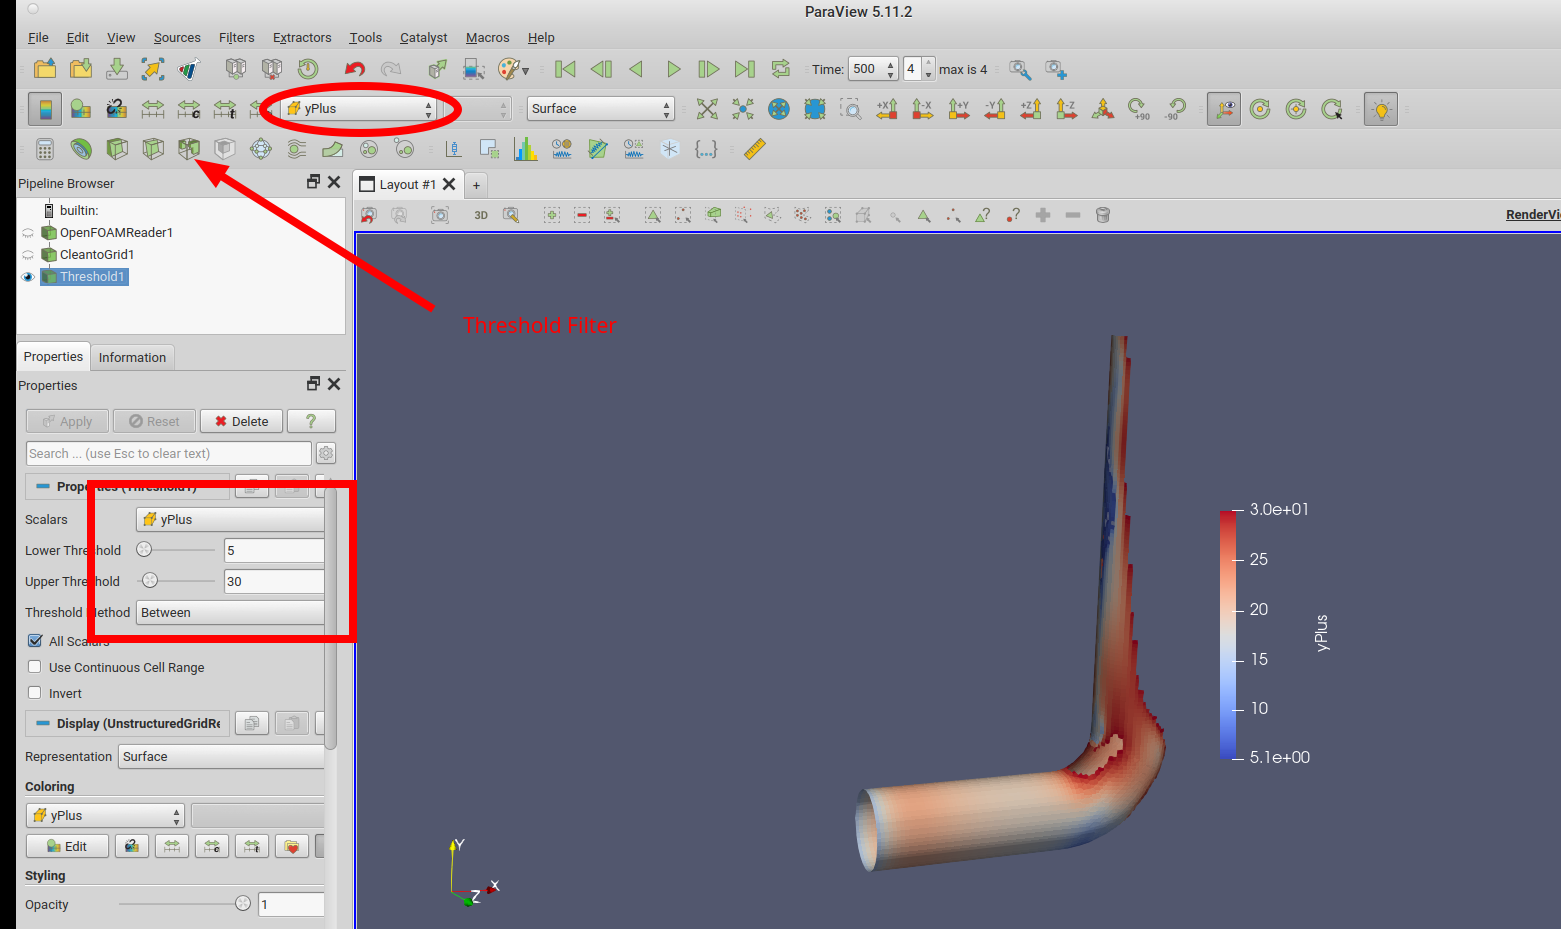
\includegraphics[width=0.7\linewidth]{yPlus1}
			\caption{Region of the wall with $y^+$ between 5 and 30.}
			\label{fig:yplus1}
		\end{figure}
		
		Note that the values of $y^+$ are very large (typically $\gtrapprox 20$), so we should significantly refine  the mesh close to the wall to get values smaller than 5. It would make the simulation very slow. 
		Alternatively, we are going to increase the size of the mesh near the wall to approach the log-law region.  
		
		\subsection{Modification of mesh to improve value of $y^+$}
		
		\item In the \texttt{FreeCAD} application, double-click in the Mesh refinement region, and change the number of layer in the boundary from 3 to 1.
		
		\item \texttt{Write} and \texttt{Run} the mesh.
		\item \texttt{Write} and \texttt{Run} the solver. Now the simulation converges much better. The values of $y^+$ are much larger, and the region where $y^+$ falls in the buffer zone is smaller. Figure \ref{fig:yplus2} shows the threshold regions for $5 < y^+ < 30$ and 
		$5 < y^+ < 25$
		
		% TODO: \usepackage{graphicx} required
		\begin{figure}
			\centering
			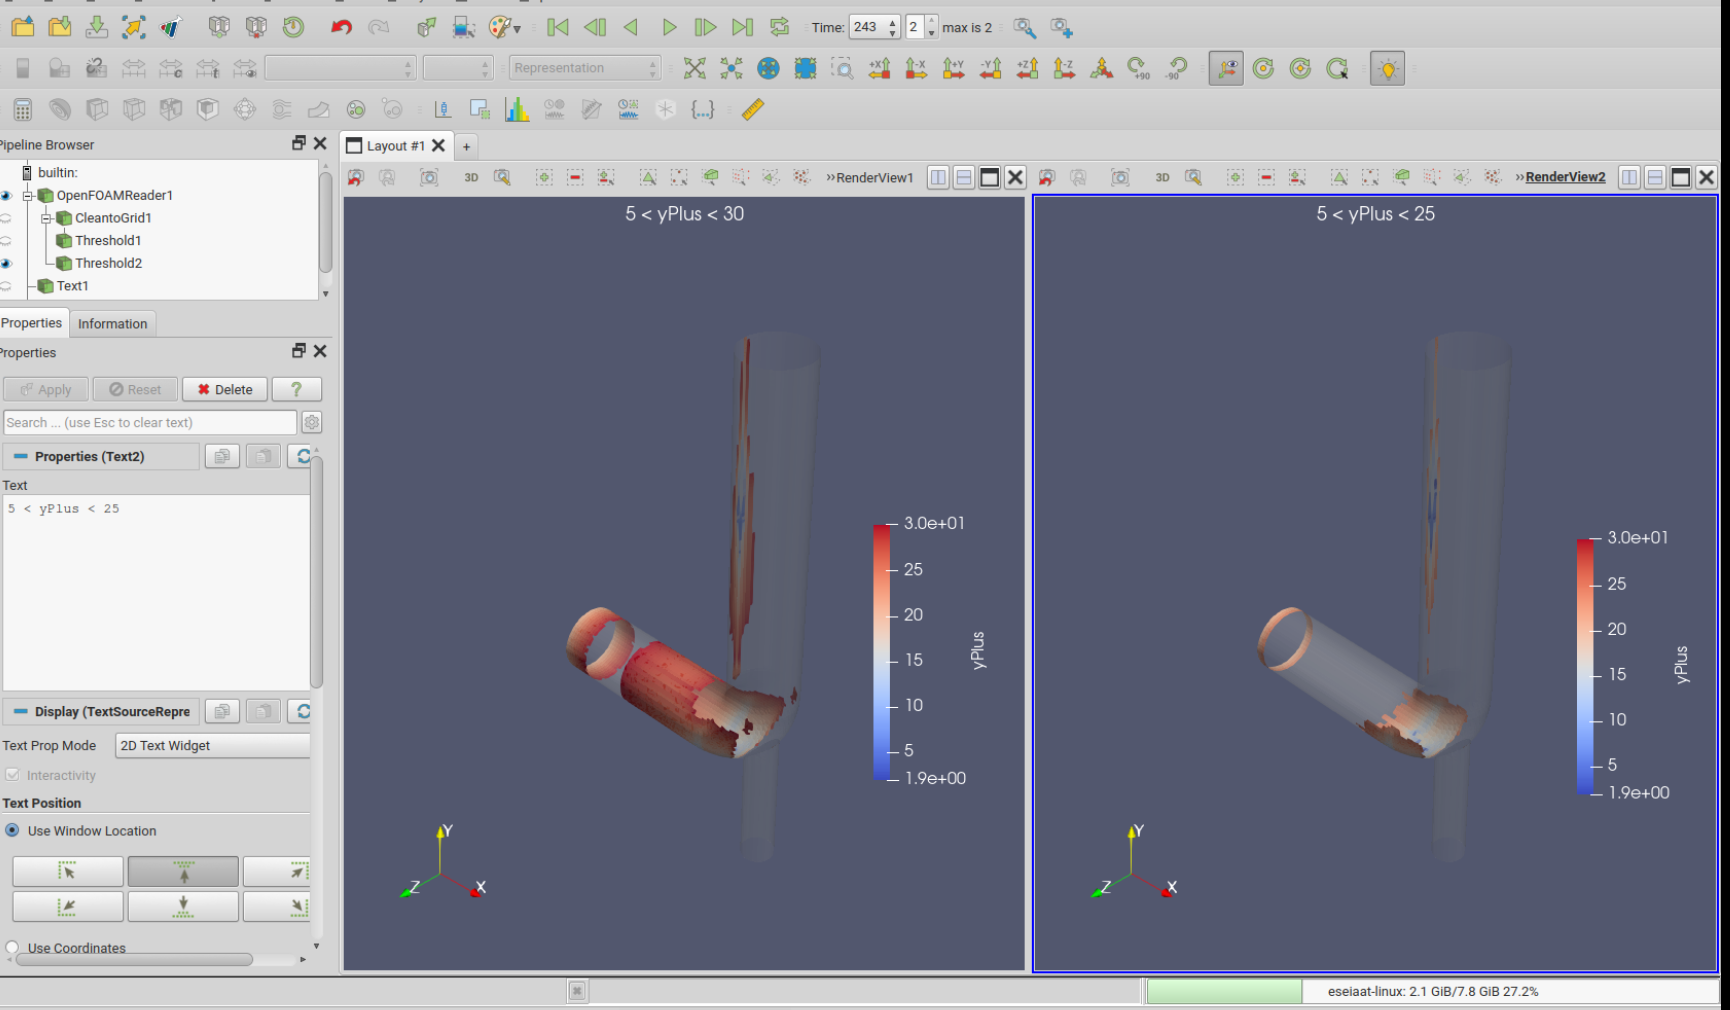
\includegraphics[width=0.7\linewidth]{yPlus2}
			\caption{Distribution of $y^+$ with new mesh}
			\label{fig:yplus2}
		\end{figure}
		
	\end{itemize}
	
	\section{Laminar simulation}
	
	\begin{itemize}
		\item Select the \texttt{Ypipe\_kOmegaSST} element and click on the menu \texttt{Edit $\rightarrow$ Duplicate selection}. Leave selected all the dependences. A new Cfd Analysis container is created in the tree. Change its name to \texttt{Ypipe\_Laminar}. 
		\item It has to be activated with a double-click.
		\item In the \texttt{CfdSolver} of this new container, change the \texttt{Input case name} to \texttt{Ypipe\_Laminar}
		\item The case has to be remeshed.
		\item \texttt{Write} and \texttt{Run} the solver. Note that a new case named \texttt{Ypipe\_Laminar}
		is created in the Tutorial\_6 folder
		\item The simulation is fast but the convergence is very bad, because the lack of a turbulence model. 
		
	\end{itemize}
	
	\section{$k-\varepsilon$ simulation}
	
\begin{itemize}
	\item Repeat the same steps than in laminar simulation but with $k-\varepsilon$ model. Change the name according to this.
	\item This simulation will need more iterations. Change the maximum number of iterations to 2000. It will take about 1000 iterations to converge.
	
\end{itemize}

\section{Note on SSTLM (Langtry-Menter 4-Equation Model)}

The SSTLM model is designed to predict laminar-to-turbulent transition and requires:

\begin{itemize}
	\item \textbf{$y^+ < 1$} at wall-adjacent cells
	\item \textbf{Much finer mesh} (typically 10-50× more cells near walls)
	\item \textbf{Significantly longer} computation time (hours instead of minutes)
\end{itemize}

\important{With our current mesh ($y^+ \gtrapprox 30$), SSTLM will produce incorrect results 
	because it cannot resolve the laminar sublayer where transition occurs. 
	For this reason, we will not run SSTLM in this tutorial, but you should be aware 
	of its existence and requirements for when you encounter transitional flows 
	(e.g., low Reynolds number airfoils, turbomachinery blades).}
	
	\section{Exercises}
	
	\subsection{Flow Rate Comparison}
	
	Using ParaView's \texttt{Integrate Variables} filter on each simulation:
	
	\begin{enumerate}
		\item Open each case in ParaView (or load them together for comparison)
		\item Select the \texttt{inletSecondary} patch
		\item Apply \texttt{Integrate Variables} filter
		\item Record the volumetric flow rate $Q = \int U \cdot dA$
		\item Create a table like Table \ref{tab:flowrates}:
		
		\begin{table}[h]
			\centering
			\begin{tabular}{|l|c|c|c|}
				\hline
				\textbf{Model} & \textbf{Flow rate (m³/s)} & \textbf{Iterations to converge} & \textbf{Notes} \\
				\hline
				Laminar & & & Unstable convergence \\
				$k$-$\varepsilon$ & & & Good convergence \\
				$k$-$\omega$ SST  & & & Very good convergence \\
				\hline
			\end{tabular}
			\caption{Flow rate comparison across turbulence models}
			\label{tab:flowrates}
		\end{table}
		
		\item Which model predicts the highest flow rate? The lowest? Why?
	\end{enumerate}
	
	\subsection{Pressure Drop: Main Inlet to Outlet}
	
	Although both have zero-gradient or fixed pressure, you can still calculate:
	
	\begin{equation*}
		\Delta p_{main-outlet} = p_{main,inlet} - p_{outlet}
	\end{equation*}
	
	Since $p_{outlet}=0$ (fixed), this becomes simply $p_{main,inlet}$.
	
	\begin{enumerate}
		\item In \texttt{ParaView}, select the \texttt{inletMain} patch.
		\item Compute the average pressure value (it will not be zero!)
		\item Compare across turbulence models:
		
		\begin{table}[h]
			\centering
			\begin{tabular}{|l|c|}
				\hline
				\textbf{Model} & \textbf{$p_{main,inlet}$ (Pa)} \\
				\hline
				Laminar & \\
				$k$-$\varepsilon$ & \\
				$k$-$\omega$ SST & \\
				\hline
			\end{tabular}
			\caption{Pressure at main inlet for different models}
			\label{tab:pressure_main}
		\end{table}
		
		\item Which model requires the highest pressure to drive the flow? Why?
	\end{enumerate}
	
\end{document}
